\documentclass[12pt]{article}
\usepackage{titling}
\usepackage{graphicx}
\usepackage{caption}
\usepackage{helvet}
\usepackage{hyperref}
\usepackage{bookmark}
\usepackage{framed}
\usepackage{listings}
\usepackage{mdframed}
\usepackage{sectsty}
\usepackage{tikz}
\newcommand{\abs}[1]{\left|#1\right|}

\renewcommand{\lstlistingname}{}

% Define font size and family for sections
\sectionfont{\fontsize{10}{12}\selectfont\renewcommand{\familydefault}{\sfdefault}}
\subsectionfont{\fontsize{10}{12}\selectfont\renewcommand{\familydefault}{\sfdefault}}
\subsubsectionfont{\fontsize{10}{12}\selectfont\renewcommand{\familydefault}{\sfdefault}}
\paragraphfont{\fontsize{10}{12}\selectfont\renewcommand{\familydefault}{\sfdefault}}
\subparagraphfont{\fontsize{10}{12}\selectfont\renewcommand{\familydefault}{\sfdefault}}
\renewcommand{\familydefault}{\rmdefault} % Reset default to Roman for title page

\usepackage[utf8]{inputenc}
\usepackage{amsmath}
\usepackage{hyperref}

\lstset{
    language=Matlab,
    basicstyle=\ttfamily\footnotesize,
    keywordstyle=\color{blue},
    commentstyle=\color{green},
    stringstyle=\color{red},
    frame=single,
    breaklines=true,
    keepspaces=true,
    showspaces=false,
    showstringspaces=false
}


\begin{document}

% Prima pagina
\begin{titlepage}
    \centering
    {\Huge \textbf{Università degli Studi di Padova} \par}
    \vspace{1cm}
    \begin{figure}[h!]
        \centering
        \includegraphics[width=0.6\textwidth]{Immagini/Logo_Università_Padova.png}
    \end{figure}
    \vspace{1.5cm}
    {\LARGE \textbf{Report about:} \par}
    {\Huge 2nd Matlab project \par}
    \vfill
    \textbf{Realized by:} \par
    Riccardo Berengan, matriculation number 2080041 \par
    Michele Dioli, matriculation number 2077629 \par
    Gabriele Di Pietro, matriculation number 2010000 \par
    \vspace{0.5cm}
\end{titlepage}
    % Change font and size for the rest of the document
    \renewcommand{\familydefault}{\sfdefault} % Set default to sans serif
    \fontsize{10}{12}\selectfont
    % Pagina introduzione
    \newpage
    \section{Introduction}
    The eigenvalues are the solutions to the equation $det(A-\lambda I) = 0$. 
    The eigenspace is the vectorial subspace generated by all the vectors and eigenvalues $\lambda$,
    together with the null vector.\\ \textit{Example:}
    \begin{align*}
        A &= \begin{bmatrix}
            4 & 2 \\
            1 & 3 \\
        \end{bmatrix}
    \end{align*}
    $det(A-\lambda I) = det\begin{bmatrix}
        4-\lambda & 2 \\
        1 & 3-\lambda \\
    \end{bmatrix} \iff (\lambda - 5)(\lambda-2) = 0 \iff \lambda_1 = 5 \lambda_2 = 2$\\
    The geometric multiplicity is the dimension of the eigenspace, associated with an eigenvalue then $\abs{n - \text{rk}(A - \lambda I)}$. Our purpose is to calculate the geometric and the algebraic multiplicities to define if a matrix is diagonalizable or not.
    \section{Calculation}
    \subsection{Multigeo Function}
    For the calculation, count the "null" values \textit{(smaller than a tolerance)} in the matrix $U$ obtained using the factorization $LU$. It can be done because:
    A blank row in $U$ means that the linear system of $(A-\lambda I)x = 0$ has a free solution, a blank row does not depend from the other rows of the matrix, the blank rows indicate that there are linear dependencies between the rows.
    The approach is to count the elements in the diagonal line that are larger than a tolerance, thus counting the matrix rank. Then subtract this number from the matrix dimension to obtain the eigenspace dimension of the eigenvalue that coincides with the geometric multiplicity.
    \subsection{Myobjective Function}
    The function \texttt{myobjective} is used to calculate the funcion $f$ and the function $g$ from a scalar value $z$ and a squared matrix $A$.\\
    The first step is to calculate the matrix $B = A - zI$, and then, by using the LU factorization using \texttt{lu(B)} in Matlab that returns  $U$, upper matrix, and the $L$ lower matrix. Then we calculate $P$, the permutation matrix. \\
    $P=\pm1$ based on the number of permutations that occurred during this process, from which we calculate the determinant matrix P. Once we found it we calculate the $B$ determinant as $det(P) \cdot \prod_{i=1}^{n} U_{ii}$, where $U_{ii}$ are the elements on the $U$ diagonal. $f = det(B)$\\
    After this the function calculates the inverse of the matrix $B$ and calculates $g$ as the inverse of the track \textit{(it sums the elements on the diagonal)} of $B$.
    \newpage

    \subsection{Multialg Funcion}
    It consider the polynomial with $m$ as the algebraic multiplicity $f(x)=(x-\lambda)^m g(x)$ and the Newton method $x_{n+1}=x_n - \frac{f(x_n)}{f'(x_n)}$ to find the roots of $g(x)$.
    We analyze the speed of convergence $f(x)=(x-\lambda)^{m-1} g(x) + (x-\lambda)^m g'(x)$\\
    $f'(x) = 0 \iff x = \lambda$, $m \geq 1$ isn't immediately the root $m(x-\lambda)^{m-1}$ and it's responsible for the speed of convergence, so the Newton method applied to a root that has multiplicity $m\geq 1$ has linear speed of convergence instead of a quadratic one.\\
    The error estimate is reduced, depending on the root multiplicity $|x_{n+1}-\lambda| \approx |x_n - \lambda|^{\frac{m-1}{m}}$\\
    $\frac{m-1}{m}$ is the speed of convergence\\ \textit{(Newton method initialized near multiple roots $\Rightarrow |e_{n+1}| \approx C|e_n|^{\frac{m-1}{m}}$)}\\
    We calculate the eigenvalue with the newton method, iterating until a specified number of iterations and/or until we reach a sensible tolerance. The function then applies the Newton method to the characteristic polynomial $f(\lambda) = det(A-\lambda I) \Rightarrow \lambda_{n+1} = \lambda_n - \frac{f(\lambda_n)}{f'(\lambda_n)}$. With this process, we find the eigenvalue.
    To calculate the algebraic multiplicity we divide the eigenvalue by the characteristic polynomial, and we count the times that we can do this division having a result different from zero.
    \section{Test}
    \subsection{File \texttt{main.m}}
    The main file allows to define a test matrix by modifying the \texttt{lambda} vector, it allows to change the starting point for the newton method \texttt{lO} and also to change the tolerance parameter \texttt{toll}.\\
    The matrix used in tests is created through the modification of the \texttt{lambda} parameter. After the definition of lambda we call the \texttt{creaJacob} function that uses \texttt{lambda} as input and it returns the Jordan block matrix as output. Then the main creates $Q$ through \texttt{Q = orth(randn(n))}, that creates an orthogonal matrix. After that, the matrix $A$ is calculated by using the following structure: $A=Q^tJQ$\\
    \newpage
    \subsection{File \texttt{test.m}}
    The \texttt{test.m} file runs some tests to verify correctness of the  \texttt{multialg} and \texttt{multigeo} functions. These function's purpose is to calculate the eigenvalues of the matrix and their algebraic and geometric multiplicities.
    The program defines a group of test cases, each with a matrix of eigenvalues that are specified by the \texttt{lambda} value, the starting point \texttt{lO} of the Newton method, and a tolerance \texttt{toll}.
    \begin{lstlisting}[language=Matlab, frame=single, caption={Test Cases}, captionpos=b]         
TestCases = {
    struct('lambda', [1,1,1,1,1,4,4,4,4,4,4,4], 'lO', 3.8, 'toll', 1e-4),
    struct('lambda', [1, 1.01, 1.02, 5, 5.01, 5.02, 10, 10.001, 10.002, 10.003], 'lO', 10.1, 'toll', 1e-4),
    struct('lambda', [1, 1.01, 1.02, 5, 5.01, 5.02, 10, 10.001, 10.002, 10.003], 'lO', 1.0125, 'toll', 1e-4),
    struct('lambda', [1,1,1,4,5,6], 'lO', 3.5, 'toll', 1e-4),
    struct('lambda', [1,1,1,4,5,6], 'lO', 3.9, 'toll', 1e-4),
    struct('lambda', [1,1,1,4,5,6,4], 'lO', 3.9, 'toll', 1e-4),
    struct('lambda', [1,1,1,4,5,6,4,4], 'lO', 3.5, 'toll', 1e-4),
    struct('lambda', [1,1,1,4,5,6,4,4,4], 'lO', 3.7, 'toll', 1e-4), 
    struct('lambda', [1,1,1,4,5,6,4,4,4,4], 'lO', 3.3, 'toll', 1e-4), 
    struct('lambda', [1,1,1,4,5,6,4,4,4], 'lO', 3.7, 'toll', 1e-4),
    struct('lambda', [1,1,1,4,5,6,4,4,4,4], 'lO', 3.5, 'toll', 1e-4),
    struct('lambda', [1,1,1,4,5,6,4,4,4,4,4], 'lO', 4.3, 'toll', 1e-4), 
    struct('lambda', [1,1,1,4,5,6,4,4,4,4,4], 'lO', 3.5, 'toll', 1e-4), 
    struct('lambda', [1,1,1,4,5,6,4,4,4,4,4,4], 'lO', 3.4, 'toll', 1e-4),
    struct('lambda', [4,4,4,4,4,4,4,4], 'lO', 0., 'toll', 1e-4),
};
    \end{lstlisting}
    \newpage
\subsubsection{Test execution}
For every test case the program runs the following steps:
    \begin{enumerate}
        \item Print the number of the test and the values of \texttt{lambda}, \texttt{lO}, and \texttt{toll}.
        \item Creates the diagonal matrix \texttt{J} with the \texttt{lambda} values and adds 1 to the elements on the diagonal to manage multiplicities.
        \item It generates a \texttt{Q} orthogonal matrix and calculates the \texttt{A} matrix as \texttt{A = Q' * J * Q}.
        \item It uses the \texttt{multialg} function to calculate the eigenvalue \texttt{l} and his algebraic multiplicity named \texttt{m}.
        \item If the Newton method converges, it calculates the geometric multiplicity, named \texttt{k}, of the eigenvalues by using the \texttt{multigeo} function.
        \item It prints the test results, including  the calculated eigenvalue, the algebraic and geometric multiplicities and a message that confirms the convergence.
    \end{enumerate}
    The program gives a detailed analysis of the results for each test, permitting a verification on the accuracy and the efficiency of the implemented functions. 
    \newpage
\begin{lstlisting}[language=Matlab, frame=single, caption={Esecuzione dei test}, captionpos=b]
for testID = 1:length(TestCases)
    fprintf('\nExecuting Test %d...\n', testID);    
    lambda = TestCases{testID}.lambda;
    fprintf('[%s]\n', sprintf('%g ', lambda));
    lO = TestCases{testID}.lO;
    fprintf('lO = %d\n', TestCases{testID}.lO);
    toll = TestCases{testID}.toll;
    fprintf('toll = %d\n', TestCases{testID}.toll);
    J = diag(lambda);
    for i = 2:length(lambda)
        if J(i,i) == J(i-1,i-1)
            J(i-1,i) = 1;
        end
    end
    n = length(lambda);
    Q = orth(randn(n)); 
    A = Q' * J * Q;
    A1 = A;
    disp(J);     
    it = 5;
    maxit = 50;
    [l, m, flag] = multialg(A, lO, toll, it, maxit);
    if flag == 1
        fprintf('Newton convergence.\nCalculated eigenvalue: %f\nEstimated algebraic multiplicity: %d\n', l, m);
        l1 = round(l);
        toll = 1e-6;
        k = multigeo(A1, l1, toll);
        fprintf('Geometric multiplicity of %f: %d\n', l1, k);
    else
        fprintf('Non-convergent Method.\n');
    end
    linea = 50;
    fprintf('%s\n', repmat('-', 1, linea));
end
\end{lstlisting}
\newpage
\subsubsection{Terminal output}
For convenience we'll print just one test case, the other ones are similar.
    \begin{framed}
    \begin{verbatim}
Executing Test 14...
[1 1 1 4 5 6 4 4 4 4 4 4 ]
lO = 3.400000e+00
toll = 1.000000e-04
     1     1     0     0     0     0     0     0     0     0     0     0
     0     1     1     0     0     0     0     0     0     0     0     0
     0     0     1     0     0     0     0     0     0     0     0     0
     0     0     0     4     0     0     0     0     0     0     0     0
     0     0     0     0     5     0     0     0     0     0     0     0
     0     0     0     0     0     6     0     0     0     0     0     0
     0     0     0     0     0     0     4     1     0     0     0     0
     0     0     0     0     0     0     0     4     1     0     0     0
     0     0     0     0     0     0     0     0     4     1     0     0
     0     0     0     0     0     0     0     0     0     4     1     0
     0     0     0     0     0     0     0     0     0     0     4     1
     0     0     0     0     0     0     0     0     0     0     0     4
        
Newton convergence.
Calculated eigenvalue: 4.000005
Estimated algebraic multiplicity: 7
Geometric multiplicity of 4.000000: 2
--------------------------------------------------
    \end{verbatim}
    \end{framed}
    \begin{center}
        \textbf{3: Tests case output}
    \end{center}
    \newpage
    \begin{figure}[htbp]
        \begin{tikzpicture}
            \node[anchor=east,inner sep=0] (img1) at (0,0) {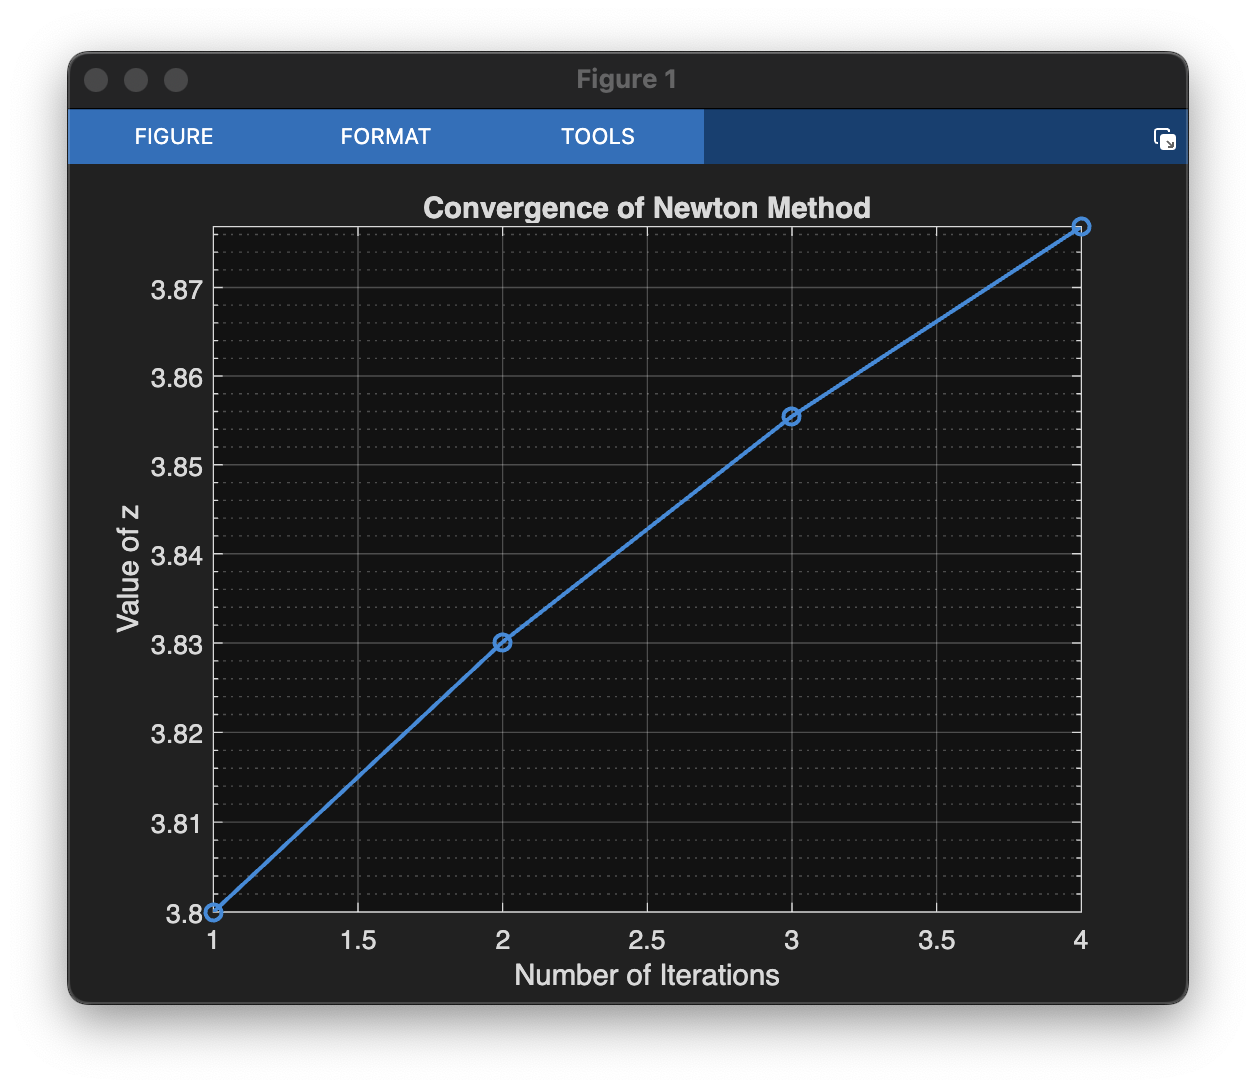
\includegraphics[width=0.5\textwidth]{Immagini/figure1.png}};
            \node[anchor=west,inner sep=0] (img2) at (0.1,0) {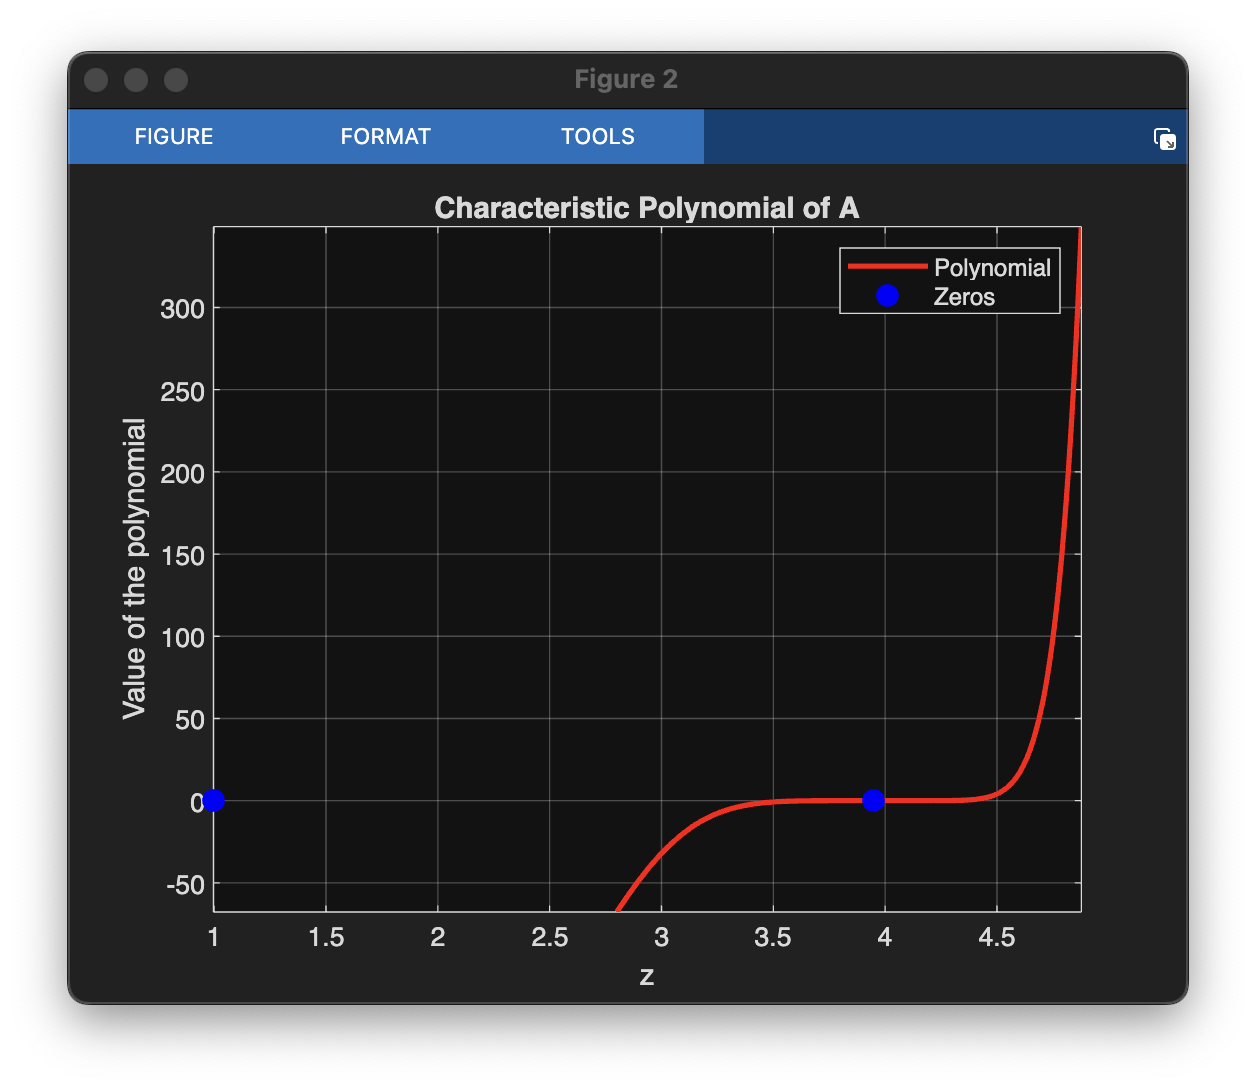
\includegraphics[width=0.5\textwidth]{Immagini/figure2.png}};
        \end{tikzpicture}
            \caption{\textit{Newton method's convergence and A polynomial}}
    \end{figure}
On some separate graphs are shown both the Newton convergence and the A polynomial.

    \section{Conclusions}
    We can say that the software manages the problem well and that it can find the eigenvalues also with far initial estimations, and the Newton method will still converge (\textit{for example}, \texttt{lO}$= 3.5$ for $\lambda = 4$). \\ 
    The software has been tested with matrices of various dimensions and with different algebraic and geometric multiplicities. In every case the Newton method is able to converge, unless the choice of the starting point is very far from the eigenvalue that we want to find.\\
\end{document}
